% 第4章第6节：本章小结。

\section{本章小结}
\label{sec:sob-summary}

本章开头的问题是：经典导数失效以后，怎样保存变化的信息，以及控制了函数和它的变化之后能得到什么。回答由一条对象链和四个分支问题组成，图~\ref{fig:sob-object-relations}把它们画在一起。

\begin{figure*}[!htb]
  \centering
  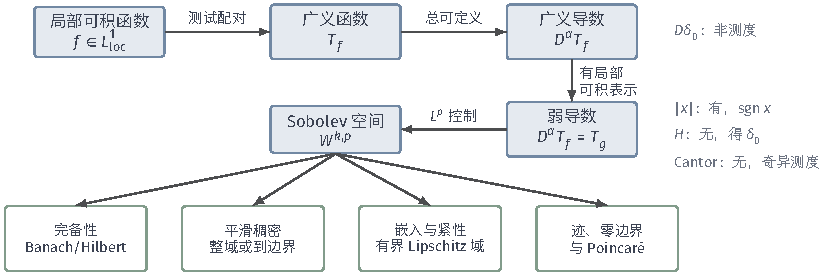
\includegraphics[width=140.6mm]{figures/02-abstract-mathematics/03-function-spaces/tikz/c4-object-relations/figure.pdf}
  \caption{本章的对象关系。上行：局部可积函数经测试配对成为广义函数，广义导数总能定义；只有当广义导数有局部可积表示时才得到弱导数，再加上$L^p$大小的控制便得到Sobolev空间。下行：Sobolev空间上分别研究的四个问题，其中嵌入、紧性与迹需要有界Lipschitz区域等条件。右侧的例子检验对象链的边界：$\delta_0$的导数不是测度，$|x|$有弱导数，阶跃与Cantor函数的广义导数分别是点质量与奇异测度。}
  \label{fig:sob-object-relations}
\end{figure*}

\paragraph{对象链及其边界}
从分部积分出发，我们把导数转移到紧支撑的光滑测试上。局部可积函数通过积分配对成为广义函数，广义导数对每个广义函数都有定义，但输出可能超出函数甚至测度的范围，$D\delta_0$就是这样。当广义导数恰好由一个局部可积函数表示时，称之为弱导数；测试函数能区分局部可积函数，所以弱导数在几乎处处意义下唯一。尖点函数$|x|$有弱导数$\operatorname{sgn}x$；阶跃函数的广义导数是$\delta_0$，Cantor函数的广义导数是集中在零测集上的奇异测度，两者都没有弱导数，尽管它们几乎处处有经典导数。在一维，弱可微恰好等价于有绝对连续代表，即能从导数积分恢复函数；导数的积分指数$p$进一步决定代表的Hölder指数$1-1/p$。把函数和直到$k$阶的弱导数的$L^p$大小同时放进范数，得到Sobolev空间$W^{k,p}$；零阶项控制水平，导数项控制变化。

\paragraph{四个问题各自的条件}
在Sobolev空间上，我们分别回答了几个不能互相代替的问题。完备性对任意开集成立，$H^k$因而是Hilbert空间，但它不提供连续代表、边界值或强收敛子列。光滑逼近分三层：磨光与弱导数交换给出局部逼近；单位分解把它拼成任意开集上的内部光滑逼近；光滑到边界的逼近需要Lipschitz边界和延拓。连续嵌入由积分指数与维数比较决定：$p<d$时得到$L^{p^*}$，$p>d$时得到Hölder连续代表，临界的$p=d\ge2$两者都差一点；缩放论证解释了$p^*=dp/(d-p)$的来源，幂函数检验了它的精确性。紧嵌入在有界Lipschitz区域上把有界序列变成$L^q$（$q<p^*$）中收敛的子列，在临界指数处因集中而失效，在无界区域上因平移逃逸而失效。边界迹把光滑函数的边界限制延拓为$H^1(\Omega)\to L^2(\partial\Omega)$的有界算子，输出是边界上的等价类；零迹函数恰好构成$H_0^1$。Poincaré不等式在排除常数方向之后，让导数单独控制函数，零边界与零均值是两种排除方式，后者还需要区域连通。

\paragraph{与后续内容的关系}
这些空间和工具为后面的问题提供了语言。第~\ref{chap:rkhs}章研究点值读取连续的Hilbert函数空间，本章一维的端点估计和$H^k$（$k>d/2$）的连续代表是那里的具体例子，而高维$H^1$在一点附近可以无界，则说明点值连续并非理所当然。在优化中，Sobolev空间用来指定目标函数的定义域，$G+H_0^1$给出保持边界值的可行扰动，紧嵌入配合弱收敛子列处理极小化序列；在微分方程与演化问题中，它们用来表达弱解。本章只建立空间、微分和边界的工具，不由这些工具直接断言某个具体问题有解。
